\newpage
\section{Введение}

С развитием техники и нашего понимания мозга возрос и интерес широкой публики к наукам о мозге, к поразительным новым открытиям и их значению для людей. В то же время исследования мозга окружает немалая шумиха, и, уж конечно, они плодят уйму неподтвержденных сведений. Кроме того, множатся мифы о мозге. Один из самых расхожих примеров — представление о том, что левое полушарие у человека «логическое», а правое «творческое». Это представление, похоже, имеет все более широкое хождение, особенно в образовательной и деловой среде. 




Это лишь один маленький пример, а таких заблуждений десятки. Поэтому мы с моим коллегой, Урсовым Эдуардом. Решили создать сервис, который помог бы любому интересующемуся разобраться с основными моментами. Мы задались задачей сделать сервис наглядным, простым и удобным, чтобы пользователю не приходилось рыскать по статьям и различным сайтам, а сразу же получить нужную информация

\begin{figure}[h]
	\center{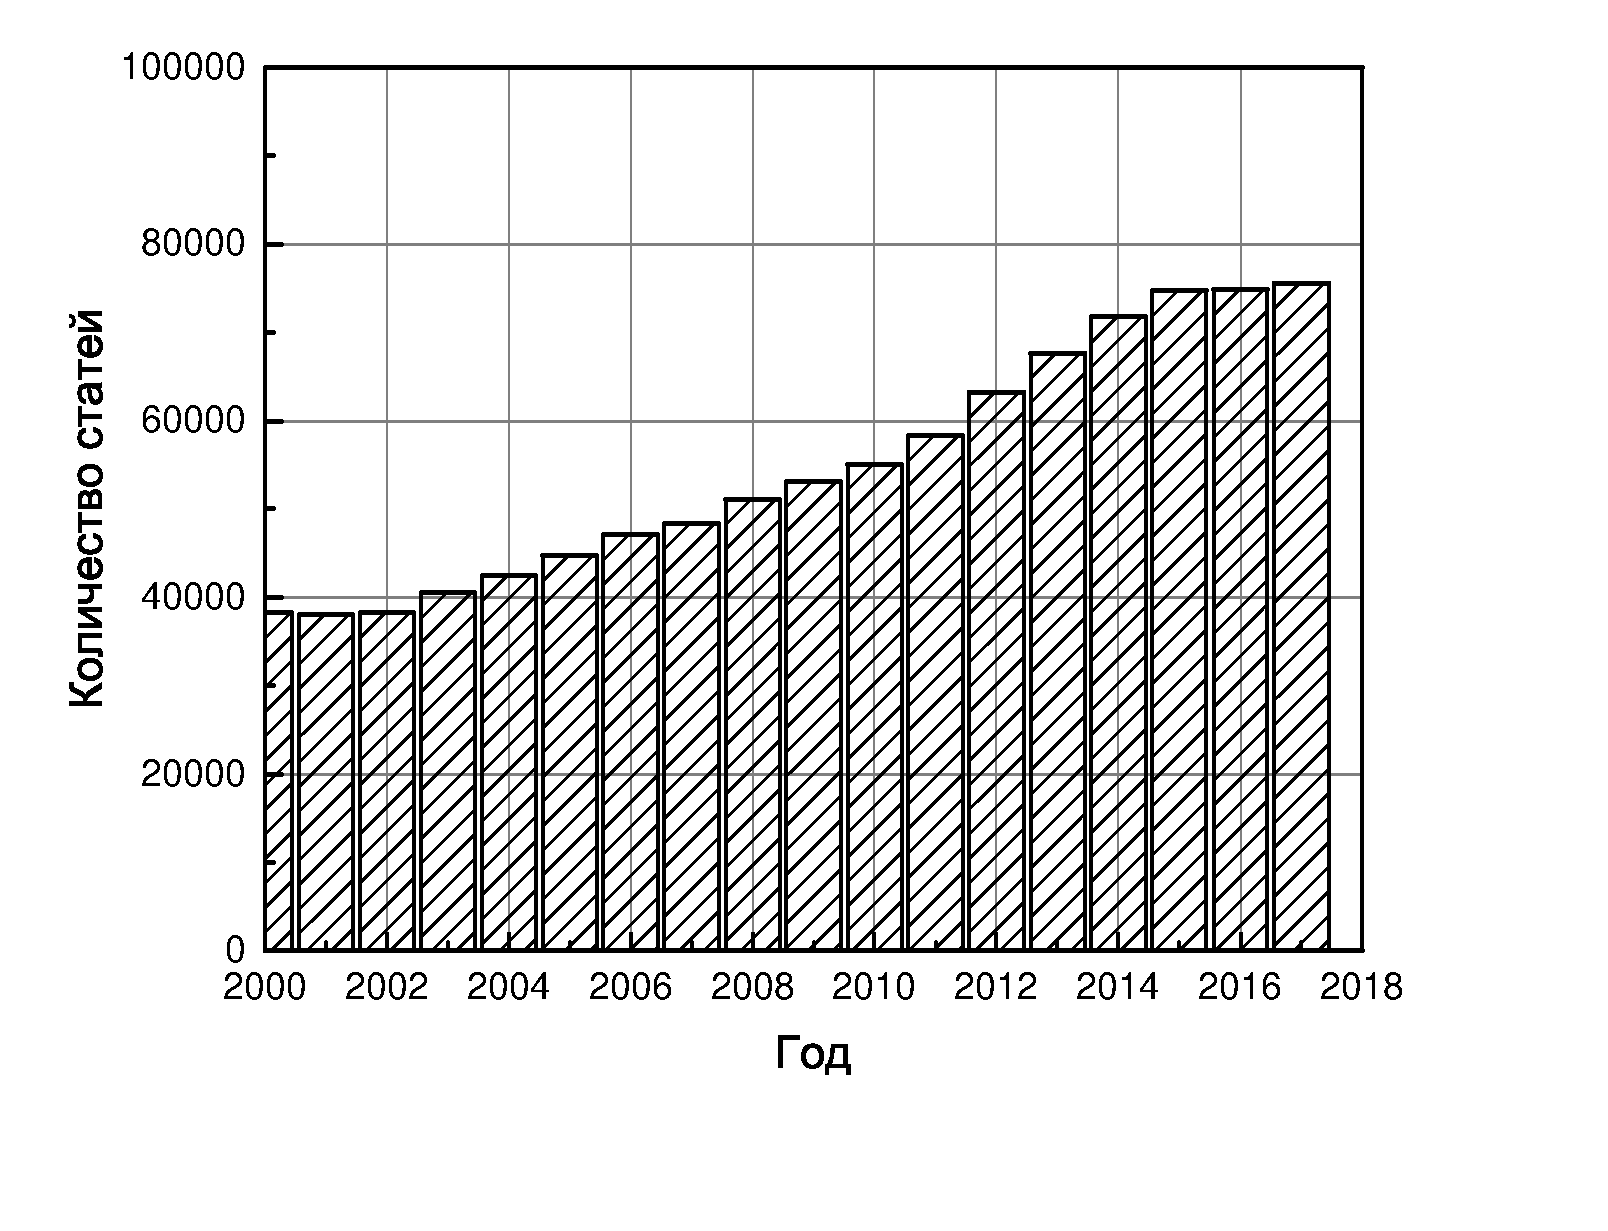
\includegraphics[width=1\linewidth]{1}}
	\caption{Зависимость количества научных статей на темы связанные с мозгом. Информация взята с ресурса  pubmed }
	\label{fig:1}
\end{figure}